\chapter{配合作用}\label{ch:b1:complexation}

向淡蓝色的硫酸铜溶液中滴入少量氨水，
立即生成淡蓝色沉淀。再滴入更多氨水，沉淀
溶解，得到颜色深邃、近乎墨蓝的溶液。酸碱与沉淀两章
都无法解释第二步。氨分子
通过\omterm{def:b1:lewis-resonance-vsepr:lewis}{孤电子对}与铜离子结合，生成了一种新物种——
\omterm{def:b1:complexation:complex}{配合物}。它比氢氧化物更稳定，颜色也不同。
\omterm{def:b1:complexation:complex}{配合物}在血液中输送氧，在叶绿素与维生素 B$_{12}$ 中容纳金属，
软化硬水，还能溶解其他物质都无法溶解的金属。
本章把\omterm{def:b1:complexation:complex}{配合物}视为水中粒子的又一种交换，
并讨论其特有的常数与图示。

\begin{recall}
\omterm{def:b1:lewis-resonance-vsepr:lewis-acid}{路易斯酸}（电子对受体）、\omterm{def:b1:lewis-resonance-vsepr:lewis-acid}{路易斯碱}（电子对给体）与
\omterm{def:b1:lewis-resonance-vsepr:lewis-acid}{配位键}已在\cref{ch:b1:lewis-resonance-vsepr}中定义。
\omterm{def:b1:predominant-reaction:predominance}{优势区域图}与\omterm{def:b1:predominant-reaction:predominant-reaction}{优势反应}法来自
\cref{ch:b1:predominant-reaction}；\omterm{def:b1:precipitation:solubility-product}{溶度积}与
沉淀生成条件来自\cref{ch:b1:precipitation}。
\end{recall}

\begin{omfigure}
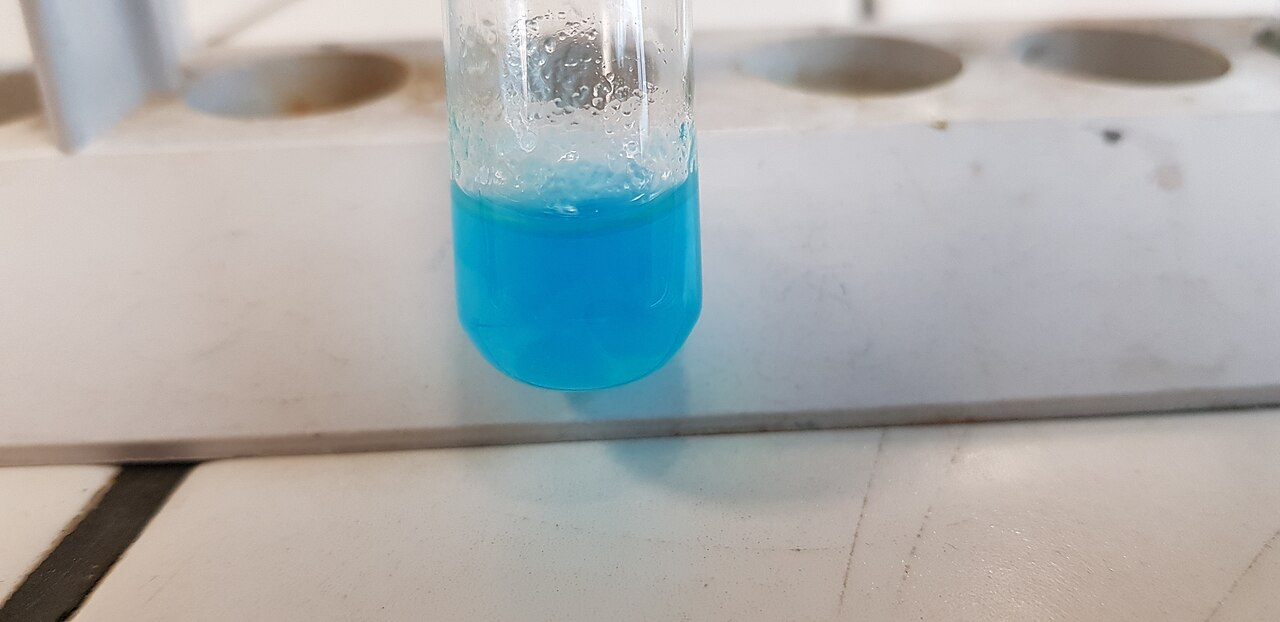
\includegraphics[height=4.2cm]{images/book2/copper-hydroxide.jpg}\hspace{0.6em}%
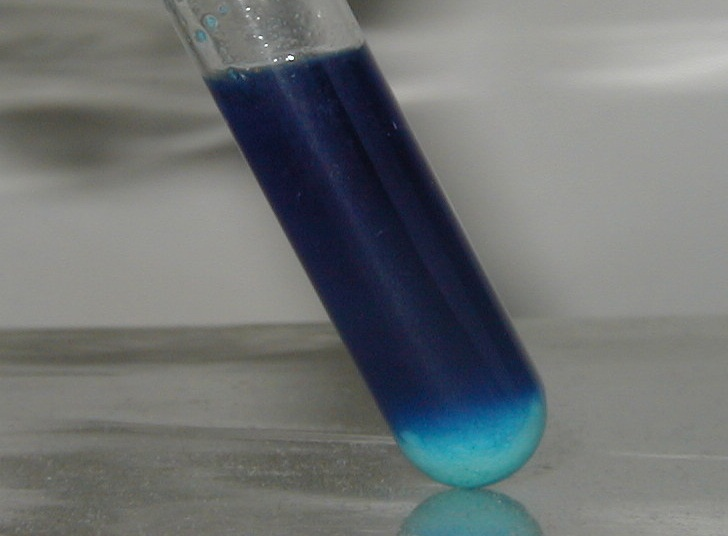
\includegraphics[height=4.2cm]{images/book2/copper-ammine.jpg}

{\small 左：淡蓝色氢氧化铜(II)悬浊液
（照片：Alvy16，CC BY 4.0）。右：加入更多氨水后，固体
溶解，生成深蓝色的四氨合铜(II)离子；试管底部仍有少量未溶的
氢氧化铜（照片：Chemicalinterest，公有领域）。
两图均取自维基共享资源。}
\end{omfigure}

\section{配合物与配体}

\begin{definition}[配合物、中心原子、配体]\label{def:b1:complexation:complex}
称\emph{配合物}\index{配合物}为由\emph{中心原子}\index{中心原子}
或离子，通常是作为\omterm{def:b1:lewis-resonance-vsepr:lewis-acid}{路易斯酸}的金属阳离子，
与作为\omterm{def:b1:lewis-resonance-vsepr:lewis-acid}{路易斯碱}的分子或离子通过\omterm{def:b1:lewis-resonance-vsepr:lewis-acid}{配位键}结合而成的粒子，
这些分子或离子即\emph{配体}\index{配体}。配合物的化学式写在
方括号内，并标明总电荷，例如 $[\ce{Cu(NH3)4}]^{2+}$、
$[\ce{Fe(CN)6}]^{4-}$、$[\ce{Ag(NH3)2}]^{+}$、$[\ce{FeSCN}]^{2+}$。
\end{definition}

\omterm{def:b1:complexation:complex}{配合物}的电荷等于中心离子与\omterm{def:b1:complexation:complex}{配体}的电荷之和：
$\mathrm{Fe^{2+}}$ 与六个 \ce{CN-} 结合，
形成 $[\ce{Fe(CN)6}]^{4-}$。\omterm{def:b1:complexation:complex}{配体}至少要有一个\omterm{def:b1:lewis-resonance-vsepr:lewis}{孤电子对}，例如 \ce{NH3}、
\ce{H2O}、\ce{OH-}、\ce{Cl-}、\ce{CN-}、\ce{SCN-}（通过 S 或 N 配位）。
事实上，水中的金属离子本身已与作为\omterm{def:b1:complexation:complex}{配体}的水分子形成\omterm{def:b1:complexation:complex}{配合物}，
如 $[\ce{Cu(H2O)6}]^{2+}$ 或 $[\ce{Fe(H2O)6}]^{3+}$；
若要形成另一种\omterm{def:b1:complexation:complex}{配合物}，就要用其他\omterm{def:b1:complexation:complex}{配体}取代这些水分子，
化学式中略去水\omterm{def:b1:complexation:complex}{配体}，正如水合质子写作 \ce{H3O+}
一样。

\begin{omfigure}
\begin{tikzpicture}[font=\small, line cap=round]
  % [Ag(NH3)2]+ : linear
  \begin{scope}
    \node (ag) at (0,0) {\ce{Ag}};
    \node (n1) at (-1.2,0) {\ce{H3N}};
    \node (n2) at (1.2,0) {\ce{NH3}};
    \draw[thick] (n1) -- (ag) -- (n2);
    \node at (0,-1.75) {$[\ce{Ag(NH3)2}]^{+}$，直线形};
  \end{scope}
  % [Cu(NH3)4]2+ : square plane in perspective
  \begin{scope}[xshift=4.3cm, every node/.style={fill=white, inner sep=1.5pt}]
    \node (cu) at (0,0) {\ce{Cu}};
    \node (a) at (-1.45,-0.5) {\ce{H3N}};
    \node (b) at (1.45,0.5) {\ce{NH3}};
    \node (c) at (0.85,-0.9) {\ce{NH3}};
    \node (d) at (-0.85,0.9) {\ce{H3N}};
    \begin{pgfonlayer}{background}
    \draw[gray, dashed] (a.center) -- (c.center) -- (b.center) -- (d.center) -- cycle;
    \end{pgfonlayer}
    \draw[thick] (cu) -- (a); \draw[thick] (cu) -- (b);
    \draw[thick] (cu) -- (c); \draw[thick] (cu) -- (d);
    \node at (0,-1.75) {$[\ce{Cu(NH3)4}]^{2+}$，平面正方形};
  \end{scope}
  % [Fe(CN)6]4- : octahedron
  \begin{scope}[xshift=9.2cm, every node/.style={fill=white, inner sep=1.5pt}]
    \node (fe) at (0,0) {\ce{Fe}};
    \node (t) at (0,1.3) {\ce{CN}};
    \node (u) at (0,-1.3) {\ce{CN}};
    \node (l) at (-1.45,-0.45) {\ce{NC}};
    \node (r) at (1.45,0.45) {\ce{CN}};
    \node (f) at (0.8,-0.8) {\ce{CN}};
    \node (k) at (-0.8,0.8) {\ce{NC}};
    \begin{pgfonlayer}{background}
    \draw[gray, dashed] (l.center) -- (f.center) -- (r.center) -- (k.center) -- cycle;
    \end{pgfonlayer}
    \foreach \x in {t,u,l,r,f,k} \draw[thick] (fe) -- (\x);
    \node at (0,-1.75) {$[\ce{Fe(CN)6}]^{4-}$，八面体};
  \end{scope}
\end{tikzpicture}

{\small 三种\omterm{def:b1:complexation:complex}{配合物}及其构型。每条线段都是由\omterm{def:b1:complexation:complex}{配体}的\omterm{def:b1:lewis-resonance-vsepr:lewis}{孤电子对}
（氨中的 N、氰根中的 C）指向金属离子的\omterm{def:b1:lewis-resonance-vsepr:lewis-acid}{配位键}；虚线勾勒出
由四个\omterm{def:b1:complexation:complex}{配体}构成的正方形。\omterm{def:b1:complexation:complex}{配合物}的构型将在
本科二年级分册中讨论。}
\end{omfigure}

\begin{definition}[多齿配体、螯合物]\label{def:b1:complexation:chelate}
同一中心离子通过其自身的多个原子同时结合的\omterm{def:b1:complexation:complex}{配体}，
称为\emph{多齿配体}\index{多齿配体}；由它形成的\omterm{def:b1:complexation:complex}{配合物}，
其中\omterm{def:b1:complexation:complex}{配体}围绕金属离子形成环，
称为\emph{螯合物}\index{螯合物}。乙二胺
\ce{H2N-CH2-CH2-NH2} 通过两个 N 原子配位，草酸根离子
\ce{C2O4^2-} 通过两个 O 原子配位，乙二胺四乙酸根离子
（\emph{EDTA}，写作 \ce{Y^4-}）通过两个 N 原子和四个 O 原子配位。
\end{definition}

\begin{omfigure}
\setchemfig{atom sep=1.9em}
\chemfig{N(-[3]-[2]C(=[1]O)-[3]O^{-})(-[5]-[6]C(=[7]O)-[5]O^{-})-[0]-[0]N(-[1]-[2]C(=[3]O)-[1]O^{-})(-[7]-[6]C(=[5]O)-[7]O^{-})}
\hspace{2.2em}
\begin{tikzpicture}[font=\small, baseline=(ca.base)]
  \node[circle, draw, thick, fill=omDef!12, inner sep=1.5pt] (ca) at (0,0) {\ce{Ca}};
  \node (n1) at (-1.15,-0.35) {N};
  \node (n2) at (0.55,-0.6) {N};
  \node (o1) at (0,1.35) {O};
  \node (o2) at (0,-1.35) {O};
  \node (o3) at (1.15,0.35) {O};
  \node (o4) at (-0.55,0.6) {O};
  \foreach \x in {n1,n2,o1,o2,o3,o4} \draw[thick, omDef] (ca) -- (\x);
  \draw[omProp, thick] (n1) .. controls (-0.57,-0.95) .. (n2);
  \draw[omProp, thick] (n1) .. controls (-1.05,0.95) .. (o1);
  \draw[omProp, thick] (n1) .. controls (-1.5,0.25) .. (o4);
  \draw[omProp, thick] (n2) .. controls (0.5,-1.6) .. (o2);
  \draw[omProp, thick] (n2) .. controls (1.5,-0.3) .. (o3);
\end{tikzpicture}

{\small 左：EDTA 离子 \ce{Y^4-}，带有两个 N 原子和四个
羧酸根基团。右：钙–EDTA \omterm{def:b1:complexation:chelate}{螯合物} $[\ce{CaY}]^{2-}$，
示意图：六个给电子原子（蓝色键）位于离子周围八面体的顶点，
其中两个 N 原子相邻，\omterm{def:b1:complexation:complex}{配体}的碳链（橙色）
闭合成五个环，每个环含五个原子，
即螯合环。}
\end{omfigure}

EDTA 离子与钙离子结合得足够牢固，
可作为水硬度滴定的试剂（见\cref{ch:b1:titration-methods}）。

\section{稳定常数与解离常数}

\begin{definition}[稳定常数与解离常数]\label{def:b1:complexation:formation-constant}
设中心离子 M、\omterm{def:b1:complexation:complex}{配体} L（略去电荷），$\mathrm{ML}_n$ 的
\emph{累积稳定常数}\index{累积稳定常数}为
$\beta_n$，即反应
$\mathrm{M} + n\,\mathrm{L} \rightleftharpoons \mathrm{ML}_n$ 的平衡常数，
\[
  \beta_n = \frac{[\mathrm{ML}_n]}{[\mathrm{M}][\mathrm{L}]^n} .
\]
称\emph{逐级稳定常数}\index{逐级稳定常数}
$K_i$ 为加入一个\omterm{def:b1:complexation:complex}{配体}时的常数，
$\mathrm{ML}_{i-1} + \mathrm{L} \rightleftharpoons \mathrm{ML}_i$ 的常数。
\emph{解离常数}\index{解离常数}为其
倒数 $K_d = 1/K_i$，且 $\mathrm{p}K_d = \log K_i$，
\omterm{def:b1:complexation:complex}{配合物}与\omterm{def:b1:complexation:complex}{配体}构成的一对，其描述方式与酸碱对完全相同，
只需以\omterm{def:b1:complexation:complex}{配体}代替质子。
\end{definition}

\begin{proposition}[累积稳定常数与逐级稳定常数]\label{prop:b1:complexation:beta-k}
$\beta_n = K_1 K_2 \cdots K_n$，即
$\log\beta_n = \sum_{i=1}^n \log K_i$ 且 $\log K_i = \log\beta_i -
\log\beta_{i-1}$（取 $\beta_0 = 1$）。
\end{proposition}

\begin{proof}
由 M 生成 $\mathrm{ML}_n$ 相当于 $n$ 次逐级加入之和，
而若干反应之和的常数等于各反应常数之积，
见\cref{ch:b1:extent-q-and-k}。直接计算：
$K_1 K_2\cdots K_n = \frac{[\mathrm{ML}]}{[\mathrm{M}][\mathrm{L}]}
\frac{[\mathrm{ML_2}]}{[\mathrm{ML}][\mathrm{L}]}\cdots
\frac{[\mathrm{ML}_n]}{[\mathrm{ML}_{n-1}][\mathrm{L}]}$，中间浓度
项相消。
\end{proof}

\begin{omfigure}
\begin{tabular}{lll}
\hline
\omterm{def:b1:complexation:complex}{配合物} & $\log\beta_n$ & $\log K_i$ \\
\hline
$[\ce{Cu(NH3)_n}]^{2+}$，$n = 1$ 至 4 & 4.10, 7.51, 10.33, 12.36 & 4.10, 3.41, 2.82, 2.03 \\
$[\ce{Ag(NH3)_n}]^{+}$，$n = 1, 2$ & 3.32, 7.22 & 3.32, 3.90 \\
$[\ce{Zn(OH)4}]^{2-}$ & $\log\beta_4 = 14.45$ & \\
$[\ce{FeSCN}]^{2+}$, $[\ce{FeF}]^{2+}$ & 2.96; 6.85 & \\
$[\ce{CaY}]^{2-}$, $[\ce{MgY}]^{2-}$, $[\ce{NiY}]^{2-}$ & 12.69, 10.90, 20.54 & \\
\hline
\end{tabular}

\smallskip
{\small \qty{25}{\celsius} 下的稳定常数。氨合、羟基、
硫氰酸根和氟\omterm{def:b1:complexation:complex}{配合物}的常数由表列标准
生成吉布斯自由能计算；EDTA 的常数取自零离子强度下经严格遴选的
数值，下文所用 EDTA 的 $\mathrm{p}K_a$ 亦然，
即 2.23、3.15、6.80 和 11.24。}
% ledger: dfg:Cu2+_ao, dfg:CuNH32+_ao, dfg:Cu_NH322+_ao, dfg:Cu_NH332+_ao, dfg:Cu_NH342+_ao, dfg:NH3_ao (computed in figdata/bachelor-1/aqueous-constants.py)
% ledger: dfg:Ag+_ao, dfg:AgNH3+_ao, dfg:Ag_NH32+_ao, dfg:Fe3+_ao, dfg:SCN-_ao, dfg:FeSCN2+_ao, dfg:F-_ao, dfg:FeF2+_ao (computed, same script)
% ledger: logb:Ca-edta, logb:Mg-edta, logb:Ni-edta, pka:edta1, pka:edta2, pka:edta3, pka:edta4
\end{omfigure}

铜氨\omterm{def:b1:complexation:complex}{配合物}的逐级常数递减，$K_1 > K_2 > K_3
> K_4$：每加入一个氨分子，剩余位点减少，使\omterm{def:b1:complexation:complex}{配合物}
对下一个氨分子的亲和力略有下降。这是通常的次序。
银是例外：$K_2 > K_1$，其推论见
周末问题。

\section{pL 标度上的优势区域}

\begin{definition}[pL 标度]\label{def:b1:complexation:pl-diagram}
对\omterm{def:b1:complexation:complex}{配体} L，$\mathrm{pL} = -\log[\mathrm{L}]$，其中 $[\mathrm{L}]$ 为
游离\omterm{def:b1:complexation:complex}{配体}的浓度。称\emph{pL 标度}\index{pL 标度}
为一条 pL 坐标轴，在其上标出中心离子
及其\omterm{def:b1:complexation:complex}{配合物}的优势区域，正如在 pH 轴上标出酸和碱的
优势区域一样。
\end{definition}

\begin{proposition}[pL 中的边界]\label{prop:b1:complexation:pl-boundaries}
对于 $\mathrm{ML}_i/\mathrm{ML}_{i-1}$ 这一对，
\[
  \mathrm{pL} = \log K_i + \log\frac{[\mathrm{ML}_{i-1}]}{[\mathrm{ML}_i]} ,
\]
于是 $\mathrm{ML}_{i-1}$ 在 $\mathrm{pL} > \log K_i$ 时占优势，
而 $\mathrm{ML}_i$ 在 $\mathrm{pL} < \log K_i$ 时占优势。当 $\log K_i$ 随 $i$ 减小时，
图形为一连串区域：$\mathrm{ML}_n$ 位于较小的 pL 处（\omterm{def:b1:complexation:complex}{配体}很多），
之后是 $\mathrm{ML}_{n-1}$，直至较大 pL 处的 M。
\end{proposition}

\begin{proof}
对 $K_i = [\mathrm{ML}_i]/([\mathrm{ML}_{i-1}][\mathrm{L}])$ 取对数：
$\log K_i = \log\frac{[\mathrm{ML}_i]}{[\mathrm{ML}_{i-1}]} + \mathrm{pL}$.
两种形式在 $\mathrm{pL} = \log K_i$ 时相等，比值
随 pL 每变化一个单位而变为十倍。$\mathrm{ML}_i$ 的区域位于
$\log K_{i+1}$ 与 $\log K_i$ 之间，只有当 $\log K_{i+1} < \log
K_i$ 时才存在。
\end{proof}

\begin{method}[绘制 pL 图]\label{met:b1:complexation:pl-diagram}
\begin{enumerate}
  \item 由 $\log\beta_n$ 依次算出各 $\log K_i$。
  \item 若它们递减，则把每个都画在 pL 轴上的边界处：
        \omterm{def:b1:complexation:complex}{配体}最多的\omterm{def:b1:complexation:complex}{配合物}在左侧（pL 较小），游离
        离子在右侧。
  \item 若某个 $\log K_{i+1} > \log K_i$，则\omterm{def:b1:complexation:complex}{配合物} $\mathrm{ML}_i$ 没有
        区域：它会自身反应，生成 $\mathrm{ML}_{i-1}$ 和
        $\mathrm{ML}_{i+1}$。去掉它，在
        $\mathrm{ML}_{i-1}$ 与 $\mathrm{ML}_{i+1}$ 之间画一条单一边界，
        位于 $\frac12(\log K_i + \log K_{i+1})$ 处。
\end{enumerate}
\end{method}

\begin{omfigure}
\begin{tikzpicture}
\begin{axis}[
  width=0.78\linewidth, height=5.2cm, xmin=0, xmax=7, ymin=0, ymax=1.05,
  axis x line=bottom, axis y line=left, xlabel={$\mathrm{pNH_3}$},
  ylabel={铜的分数},
  tick label style={font=\small}, label style={font=\small}]
\addplot[omThm, thick] table[x=pL, y=M] {figdata/out/bachelor-1-ammine-distribution-copper.dat};
\addplot[omProp, thick] table[x=pL, y=ML] {figdata/out/bachelor-1-ammine-distribution-copper.dat};
\addplot[omMeth, thick] table[x=pL, y=ML2] {figdata/out/bachelor-1-ammine-distribution-copper.dat};
\addplot[black!60, thick] table[x=pL, y=ML3] {figdata/out/bachelor-1-ammine-distribution-copper.dat};
\addplot[omDef, very thick] table[x=pL, y=ML4] {figdata/out/bachelor-1-ammine-distribution-copper.dat};
\node[omDef, font=\small, anchor=west] at (axis cs:0.15,0.78) {$n = 4$};
\node[black!60, font=\small] at (axis cs:2.42,0.63) {3};
\node[omMeth, font=\small] at (axis cs:3.12,0.55) {2};
\node[omProp, font=\small] at (axis cs:3.76,0.58) {1};
\node[omThm, font=\small, anchor=east] at (axis cs:6.9,0.84) {\ce{Cu^2+}};
\end{axis}
\end{tikzpicture}

\begin{tikzpicture}[font=\small, x=1.25cm]
  \draw[->, thick] (0,0) -- (7.2,0) node[right] {$\mathrm{pNH_3}$};
  \foreach \x/\l in {2.03/2.03, 2.82/2.82, 3.41/3.41, 4.10/4.10}
    \draw (\x,0.12) -- (\x,-0.12) node[below] {\l};
  \node[above] at (1.0,0.08) {$[\ce{Cu(NH3)4}]^{2+}$};
  \node[above, font=\scriptsize] at (2.42,0.08) {3};
  \node[above, font=\scriptsize] at (3.12,0.08) {2};
  \node[above, font=\scriptsize] at (3.76,0.08) {1};
  \node[above] at (5.6,0.08) {\ce{Cu^2+}};
  \begin{scope}[yshift=-1.25cm]
  \draw[->, thick] (0,0) -- (7.2,0) node[right] {$\mathrm{pNH_3}$};
  \draw (3.61,0.12) -- (3.61,-0.12) node[below] {3.61};
  \draw[dotted] (3.32,0.3) -- (3.32,-0.1); \draw[dotted] (3.90,0.3) -- (3.90,-0.1);
  \node[above] at (1.6,0.08) {$[\ce{Ag(NH3)2}]^{+}$};
  \node[above] at (5.4,0.08) {\ce{Ag+}};
  \end{scope}
\end{tikzpicture}

{\small 上图：铜（II）以 \ce{Cu^2+} 及
$[\ce{Cu(NH3)_n}]^{2+}$（$n = 1$ 至 4）形式存在的分数，随 $\mathrm{pNH_3}$ 变化。中图：
铜氨\omterm{def:b1:complexation:complex}{配合物}的\omterm{def:b1:predominant-reaction:predominance}{优势区域图}，边界位于
$\log K_i$ 处。下图：银，其中 $\log K_2 = 3.90 > \log K_1 = 3.32$
（虚线）：$[\ce{AgNH3}]^{+}$ 无区域，单一边界位于
$\frac12\log\beta_2 = 3.61$ 处。}
\end{omfigure}

\begin{example}[\texorpdfstring{\qty{0.010}{mol/L}}{0.010 mol/L} 氨水中的铜]\label{ex:b1:complexation:cu}
游离 $[\ce{NH3}] = \qty{0.010}{mol/L}$ 时，$\mathrm{pNH_3} = 2.0$ 位于
$[\ce{Cu(NH3)3}]^{2+}$ 的区域内，但靠近 2.03 处的
与 $[\ce{Cu(NH3)4}]^{2+}$ 的边界，二者几乎相等。各组分的分数
正比于 $\beta_n[\ce{NH3}]^n = 10^{\log\beta_n - 2n}$，即
$1 : 10^{2.10} : 10^{3.51} : 10^{4.33} : 10^{4.36}$，故 \qty{48}{\percent} 为
$[\ce{Cu(NH3)4}]^{2+}$，\qty{45}{\percent} 为 $[\ce{Cu(NH3)3}]^{2+}$，
\qty{7}{\percent} 为 $[\ce{Cu(NH3)2}]^{2+}$，几乎没有游离的 \ce{Cu^2+}。
\end{example}

\section{竞争}

一个\omterm{def:b1:complexation:complex}{配体}可被两种金属离子争夺，一个金属离子也可被两个\omterm{def:b1:complexation:complex}{配体}争夺，
二者还都参与沉淀平衡和酸–碱平衡。
每一种竞争都是一个新的反应，其常数由
已知常数组合而成；
\cref{ch:b1:predominant-reaction}中的主反应方法原样适用。

\begin{example}[铁（III）的两种配体]\label{ex:b1:complexation:scn-f}
向铁（III）溶液中滴入一滴硫氰根，生成血红色的
$[\ce{FeSCN}]^{2+}$；氟离子使其褪色：
\[
  [\ce{FeSCN}]^{2+} + \ce{F-} \rightleftharpoons [\ce{FeF}]^{2+} + \ce{SCN-},
  \qquad K = \frac{\beta(\ce{FeF})}{\beta(\ce{FeSCN})} = 10^{6.85 - 2.96} =
  10^{3.89} .
\]
稳定性较强（$\beta$ 较大）的\omterm{def:b1:complexation:complex}{配合物}夺得金属离子，
正如较强的酸把质子让给较强的碱。
\end{example}

\begin{proposition}[配合作用与沉淀的竞争]\label{prop:b1:complexation:competition-precipitation}
固体 MX 在\omterm{def:b1:complexation:complex}{配体} L 中溶解，反应为
$\mathrm{MX(s)} + n\,\mathrm{L} \rightleftharpoons \mathrm{ML}_n + \mathrm{X}$,
其平衡常数为 $K = \beta_n K_s$。若\omterm{def:b1:complexation:complex}{配合物}是溶液中 M 的唯一存在形式，
且游离\omterm{def:b1:complexation:complex}{配体}浓度为 $[\mathrm{L}]$，则
\omterm{def:b1:precipitation:solubility}{溶解度}为 $s = \sqrt{K}\,[\mathrm{L}]^{n/2}$。
\end{proposition}

\begin{proof}
该反应是溶解（常数 $K_s$）与
$\mathrm{ML}_n$ 生成（$\beta_n$）之和。饱和时 $[\mathrm{ML}_n]
= [\mathrm{X}] = s$ 且 $K = s^2/[\mathrm{L}]^n$。
\end{proof}

\begin{method}[用配合作用溶解沉淀]\label{met:b1:complexation:dissolve-precipitate}
\begin{enumerate}
  \item 将溶解反应写成生成\omterm{def:b1:complexation:complex}{配合物}的形式，并计算
        $K = \beta_n K_s$.
  \item 若 $K$ 较大，只要存在足量\omterm{def:b1:complexation:complex}{配体}，溶解即为定量的；
        若其值较小，则计算
        溶解所给定量固体所需的游离\omterm{def:b1:complexation:complex}{配体}浓度：
        $[\mathrm{L}]^n = s^2/K$.
  \item 加入\omterm{def:b1:complexation:complex}{配合物}中结合的\omterm{def:b1:complexation:complex}{配体} $n s$，
        即得需引入的\omterm{def:b1:complexation:complex}{配体}总量。
  \item 检验游离金属离子可以忽略：$[\mathrm{M}] = K_s/s
        \ll s$.
\end{enumerate}
\end{method}

在氨水中，氯化银（$K = 10^{7.22 - 9.75} = 10^{-2.53}$）
在中等浓度的溶液中溶解，而碘化银
（$K = 10^{-8.85}$）则不溶解。周末问题借此
区分这些卤化物。

\begin{proposition}[配合作用与酸度的对抗]\label{prop:b1:complexation:ligand-acidity}
若\omterm{def:b1:complexation:complex}{配体} $\mathrm{L}$ 为某酸 $\mathrm{HL}$ 的碱（还可能有更多质子化形式），
则未与金属结合的\omterm{def:b1:complexation:complex}{配体}中，仅比例为 $[\mathrm{L}]/c_L =
1/\alpha$ 的部分可供使用，其中
\[
  \alpha = 1 + \frac{[\ce{H3O+}]}{K_{an}} + \frac{[\ce{H3O+}]^2}{K_{an}K_{a(n-1)}}
  + \cdots
\]
（$K_{an}$ 为最后一级\omterm{def:b1:predominant-reaction:acidity-constant}{酸度常数}）。固定 pH 时，配合作用的表现
如同其常数为\emph{条件}常数
$\beta' = \beta/\alpha$，pH 越低则其值越小。
\end{proposition}

\begin{proof}
未与金属结合的\omterm{def:b1:complexation:complex}{配体}分布于 L、HL、\ce{H2L} 等形式之间，
其中 $[\mathrm{HL}] = [\mathrm{L}][\ce{H3O+}]/K_{an}$，对更高级的形式亦有类似的
关系（见\cref{ch:b1:predominant-reaction}）。求和得 $c_L = \alpha[\mathrm{L}]$，
又 $\beta = [\mathrm{ML}]/([\mathrm{M}][\mathrm{L}]) =
\alpha[\mathrm{ML}]/([\mathrm{M}]c_L)$，因此 $[\mathrm{ML}]/([\mathrm{M}]c_L)
= \beta/\alpha$.
\end{proof}

对于 pH 10 时的 EDTA，$\alpha = 1 + 10^{11.24 - 10} + 10^{11.24 + 6.80 - 20}
= 18.4$，故钙\omterm{def:b1:complexation:complex}{配合物}的 $\log\beta' = 12.69 - 1.26 = 11.43$；
pH 为 7 时降至 8.24（见\cref{exo:b1:complexation:9}）。这正是
钙的 EDTA 滴定总在 pH 10 的氨\omterm{def:b1:predominant-reaction:buffer}{缓冲溶液}中进行的原因。
氨同样是碱：在酸中它变为 \ce{NH4+}，不再有\omterm{def:b1:lewis-resonance-vsepr:lewis}{孤电子对}，
氨\omterm{def:b1:complexation:complex}{配合物}随之分解。在氯离子存在下向
$[\ce{Ag(NH3)2}]^{+}$ 中加入硝酸，便重新生成白色
氯化银沉淀。

照相定影液对银离子采用的是另一种\omterm{def:b1:complexation:complex}{配体}，
即硫代硫酸根离子 \ce{S2O3^2-}：它们溶解
未受光照的卤化银，使底片不再变暗。
其常数不在本册数据之中；氨与氯化银的反应
表现出同样的化学性质。

\section{练习}

\begin{exercise}[$\star$]\label{exo:b1:complexation:1}
对每一\omterm{def:b1:complexation:complex}{配合物}，给出中心离子、其电荷、\omterm{def:b1:complexation:complex}{配体}，以及
每个\omterm{def:b1:complexation:complex}{配体}的配位原子：$[\ce{Cu(NH3)4}]^{2+}$，
$[\ce{Fe(CN)6}]^{4-}$, $[\ce{Fe(CN)6}]^{3-}$, $[\ce{Ag(NH3)2}]^{+}$,
$[\ce{FeSCN}]^{2+}$, $[\ce{Zn(OH)4}]^{2-}$, $[\ce{CaY}]^{2-}$.
\end{exercise}

\begin{exercise}[$\star$]\label{exo:b1:complexation:2}
由铜氨\omterm{def:b1:complexation:complex}{配合物}的 $\log\beta_n$，计算四个 $\log K_i$
及四个 $\mathrm{p}K_d$。写出与
最后一个 $\mathrm{p}K_d$ 相对应的解离反应。
\end{exercise}

\begin{exercise}[$\star$]\label{exo:b1:complexation:3}
画出铜氨\omterm{def:b1:complexation:complex}{配合物}的 pL 图。在
$[\ce{NH3}] = 1.0$、\num{3.2e-3}、\num{3.2e-4} 与
\qty{1.0e-5}{mol/L}时，哪种铜物种占优势？
\end{exercise}

\begin{exercise}[$\star$]\label{exo:b1:complexation:4}
某溶液中含铁（III）\qty{1.0e-3}{mol/L}，硫氰酸根
浓度为 \qty{0.10}{mol/L}。忽略已结合的硫氰酸根，求
铁以 $[\ce{FeSCN}]^{2+}$ 形式存在的比例。
\end{exercise}

\begin{exercise}[$\star\star$]\label{exo:b1:complexation:5}
证明：在金属离子 M 及其\omterm{def:b1:complexation:complex}{配合物}
$\mathrm{ML}_n$ 的溶液中，$\mathrm{ML}_n$ 所占的分数为
$\beta_n[\mathrm{L}]^n / \sum_{k} \beta_k[\mathrm{L}]^k$。并证明，
若仅有 $\mathrm{ML}_{i-1}$、$\mathrm{ML}_i$ 与 $\mathrm{ML}_{i+1}$ 大量存在，则
$\mathrm{ML}_i$ 的分数在
$[\mathrm{ML}_{i-1}] = [\mathrm{ML}_{i+1}]$ 处最大，此时
$\mathrm{pL} = \frac12(\log K_i + \log K_{i+1})$，并计算
$[\ce{Cu(NH3)2}]^{2+}$ 对应的 pNH3。
\end{exercise}

\begin{exercise}[$\star\star$]\label{exo:b1:complexation:6}
向\cref{exo:b1:complexation:4}中的红色溶液加入氟化钠，
直至游离 $[\ce{F-}] = \qty{0.010}{mol/L}$，计算
\omterm{def:b1:complexation:complex}{配体}交换的常数，以及比值 $[\ce{FeF^2+}]/[\ce{FeSCN^2+}]$。
会观察到什么现象？
\end{exercise}

\begin{exercise}[$\star\star$]\label{exo:b1:complexation:7}
向 $[\ce{MgY}]^{2-}$ 溶液中加入等物质的量的钙离子，
写出交换反应，计算其常数，以及
被释放出的镁的分数。
\end{exercise}

\begin{exercise}[$\star\star$]\label{exo:b1:complexation:8}
氧化银 \ce{Ag2O} 是一种棕色固体：\ce{Ag2O(s) + H2O <=> 2Ag+ + 2OH-}
其 $\mathrm{p}K = 15.43$。写出其在氨水中溶解生成
$[\ce{Ag(NH3)2}]^{+}$ 的反应，计算其常数，并说明为何棕色
由少量氨加入硝酸银中所生成的沉淀，
会在过量的氨中溶解。
\end{exercise}

\begin{exercise}[$\star\star$]\label{exo:b1:complexation:9}
计算 $\alpha$ 及条件常数 $\log\beta'$，对象为 $[\ce{CaY}]^{2-}$，
分别在 pH 10 与 pH 7 时求值（见\cref{prop:b1:complexation:ligand-acidity}）。
若要求条件常数至少为 $10^{10}$，
为何在中性溶液中用 EDTA 滴定钙不可行？
\end{exercise}

\begin{exercise}[$\star\star\star$]\label{exo:b1:complexation:10}
氧化铜 \ce{CuO} 是氢氧化铜久置后转变成的固体；
溶解平衡 \ce{CuO(s) + H2O <=> Cu^2+ + 2OH-} 的 $\mathrm{p}K = 20.64$。
\begin{enumerate}
  \item 写出 \ce{CuO} 在氨水中溶解生成
        $[\ce{Cu(NH3)4}]^{2+}$ 的反应，并计算其常数。
  \item 仅含 \qty{1.0}{mol/L} 氨水时，pH 由氨决定
        （$\mathrm{p}K_a(\ce{NH4+}) = 9.25$）。计算该 pH 及
        溶解的铜的浓度。
  \item 对氨与氯化铵的\omterm{def:b1:predominant-reaction:buffer}{缓冲溶液}，同样求解，
        二者浓度均为 \qty{1.0}{mol/L}，并得出结论。
\end{enumerate}
\end{exercise}

\begin{exercise}[$\star\star\star$]\label{exo:b1:complexation:11}
银与氨。
\begin{enumerate}
  \item 证明 $[\ce{AgNH3}]^{+}$ 会发生自身反应，
        \ce{2[AgNH3]+ <=> Ag+ + [Ag(NH3)2]+}，并计算其常数。
  \item 求银以
        $[\ce{AgNH3}]^{+}$ 形式存在的最大分数，以及该分数出现时的 pNH3。
\end{enumerate}
\end{exercise}

\begin{exercise}[$\star\star\star$]\label{exo:b1:complexation:12}
一种 EDTA 溶液，在高 pH 下含 \qty{0.10}{mol/L} 的 \ce{Y^4-}，用于
溶解碳酸钙水垢。
\begin{enumerate}
  \item 写出该反应并计算其常数。
  \item 一升溶液可溶解多少质量的碳酸钙？
  \item 为何溶液必须呈碱性？（碳酸根与 EDTA 离子
        均为碱。）
\end{enumerate}
\end{exercise}

\section{问题：氨与三种卤化银}

\begin{problem}[{周末问题——银的氨配合物及其倒数常数，
氯化银、溴化银和碘化银在氨中的溶解，
确证试验，以及溶解一克氯化银
所需的最少氨量}]
\label{pb:b1:complexation:1}
某分析人员有三种白色至黄色的沉淀，需判断
哪一种分别是氯化银、溴化银和碘化银；随后她必须
在 \qty{1.00}{L} 中溶解 \qty{1.0}{g} 氯化银，
所用氨应尽量少。\qty{25}{\celsius} 下的数据：$\log\beta_1 = 3.32$ 和
$\log\beta_2 = 7.22$（银的氨\omterm{def:b1:complexation:complex}{配合物}）；$\mathrm{p}K_s$（\ce{AgCl}）
为 9.75，\ce{AgBr} 为 12.27，\ce{AgI} 为 16.07；$\mathrm{p}K_a(\ce{NH4+}) = 9.25$；
摩尔质量：\ce{AgCl} \qty{143.4}{g/mol}、\ce{AgBr} \qty{187.8}{g/mol}、
\ce{AgI} \qty{234.8}{g/mol}。

\medskip
\noindent\textbf{第一部分——银的氨\omterm{def:b1:complexation:complex}{配合物}。}
\begin{enumerate}
  \item 写出 $[\ce{AgNH3}]^{+}$ 和
        $[\ce{Ag(NH3)2}]^{+}$ 的生成反应，以及 $\beta_1$ 与 $\beta_2$ 的表达式。
  \item 计算 $\log K_1$ 与 $\log K_2$。
  \item 若简单地以这两条边界画出 pL 图，
        其中存在什么问题？
  \item 写出 $[\ce{AgNH3}]^{+}$ 的自身反应，并计算
        其常数。
  \item 画出正确的图；其唯一边界位于何处？
  \item 当 $[\ce{NH3}] = \qty{0.10}{mol/L}$ 时，计算
        $[\ce{Ag(NH3)2+}]/[\ce{Ag+}]$。
  \item 给出总\omterm{def:b1:complexation:formation-constant}{解离常数} $\mathrm{p}K_d$，
        其对应于 $[\ce{Ag(NH3)2}]^{+}$ 的解离。
\end{enumerate}

\medskip
\noindent\textbf{第二部分——氯化银在氨中的溶解。}
\begin{enumerate}[resume]
  \item 写出 \ce{AgCl} 在氨中溶解的反应，并计算其
        常数。
  \item 将\omterm{def:b1:precipitation:solubility}{溶解度} $s$ 表示为游离氨浓度的函数，
        并计算 $[\ce{NH3}] = \qty{1.0}{mol/L}$ 时的值。
  \item 与纯水相比，\omterm{def:b1:precipitation:solubility}{溶解度}增大了
        多少？
  \item 此时一升溶液可溶解多少质量的氯化银？
  \item 验证游离的 \ce{Ag+} 可忽略不计。
  \item 现引入的氨总浓度为 \qty{1.0}{mol/L}。计入
        已结合的氨，重新计算 $s$。
  \item 氨是一种碱；试说明在此溶液中
        为何可忽略其质子化。
\end{enumerate}

\medskip
\noindent\textbf{第三部分——溴化银与碘化银。}
\begin{enumerate}[resume]
  \item 计算 \ce{AgBr} 在氨中溶解的常数。
  \item 计算 \ce{AgBr} 在 \qty{1.0}{mol/L} 游离氨中的\omterm{def:b1:precipitation:solubility}{溶解度}，
        分别以 \unit{mol/L} 与 \unit{g/L} 表示。
  \item 同理求 \ce{AgI} 的\omterm{def:b1:precipitation:solubility}{溶解度}，以 \unit{mg/L} 表示。
  \item 由此推断鉴别三种沉淀的方法。
  \item 需要多大的游离氨浓度，才能在
        \qty{1.00}{L} 中溶解 \qty{1.0}{g} \ce{AgBr}？
  \item 对 \qty{1.0}{g} \ce{AgI} 同样求解，并加以评论。
\end{enumerate}

\medskip
\noindent\textbf{第四部分——一克氯化银。}
\begin{enumerate}[resume]
  \item 向氯化银的氨溶液中加入硝酸，
        写出总反应并计算其常数。分析者
        会观察到什么现象？
  \item 需要多大的游离氨浓度，才能在
        \qty{1.00}{L} 中溶解 \qty{1.0}{g} \ce{AgCl}？
  \item \omterm{def:b1:complexation:complex}{配合物}中结合了多少氨？
  \item 验证此溶液中游离的 \ce{Ag+} 可忽略不计。
  \item 最低的氨总浓度是多少，才能溶解
        \qty{1.0}{g} 氯化银（溶于 \qty{1.00}{L}）？
\end{enumerate}
\end{problem}
